\documentclass[a4paper,12pt]{article}


%%% Работа с русским языком
\usepackage{cmap}					% поиск в PDF
\usepackage[T2A]{fontenc}			% кодировка
\usepackage[utf8]{inputenc}		% кодировка исходного текста
\usepackage[russian]{babel}	% локализация и переносы
%\usepackage{pscyr}
%\renewcommand{\rmdefault}{ftm}
%%% Дополнительная работа с математикой
\usepackage{amsmath,amsfonts,amssymb,amsthm,mathtools} % AMS
%% Номера формул
%\mathtoolsset{showonlyrefs=true} % Показывать номера только у тех формул, на которые есть \eqref{} в тексте.
%\usepackage{leqno} % Нумерация формул слева
%\usepackage{rumathgrk1}
%% Перенос знаков в формулах (по Львовскому)
\newcommand*{\hm}[1]{#1\nobreak\discretionary{}
	{\hbox{$\mathsurround=0pt #1$}}{}}
%\usepackage{glonti}
%%% Работа с картинками
\usepackage{graphicx}  % Для вставки рисунков
\graphicspath{{images/}{images2/}}  % папки с картинками
\usepackage{wrapfig} % Обтекание рисунков текстом
\addto\captionsrussian{\def\refname{Список используемой литературы}}
%%% Работа с таблицами
\usepackage{array,tabularx,tabulary} % Дополнительная работа с таблицами
\usepackage{longtable}  % Длинные таблицы
\usepackage{multirow} % Слияние строк в таблице
%%% Теоремы
\theoremstyle{plain} % Это стиль по умолчанию, его можно не переопределять.
\newtheorem{theorem}{Теорема}[section]
\newtheorem{proposition}[theorem]{Утверждение}

\theoremstyle{definition} % "Определение"
\newtheorem{corollary}{Следствие}[theorem]
\newtheorem{problem}{Задача}[section]

\theoremstyle{remark} % "Примечание"
\newtheorem*{nonum}{Решение}
%\pagestyle{empty}
%%% Страница
\usepackage{extsizes} % Возможность сделать 14-й шрифт
\usepackage{geometry} % Простой способ задавать поля
\geometry{top=20mm}
%\geometry{bottom=35mm}
\geometry{left=25mm}
\geometry{right=20mm}
\setlength{\parindent}{1.1cm}

\usepackage{setspace} % Интерлиньяж
\onehalfspacing % Интерлиньяж 1.5
% \doublespacing % Интерлиньяж 2
%\singlespacing % Интерлиньяж 1

\usepackage{lastpage} % Узнать, сколько всего страниц в документе.
\usepackage[usenames]{color}
\usepackage{colortbl}
\renewcommand{\baselinestretch}{1.05}
\usepackage{hyperref}
\usepackage[usenames,dvipsnames,svgnames,table]{xcolor}
\hypersetup{				% Гиперссылки
	unicode=true,           % русские буквы в раздела PDF
	pdftitle={Заголовок},   % Заголовок
	pdfauthor={Автор},      % Автор
	pdfsubject={Тема},      % Тема
	pdfcreator={Создатель}, % Создатель
	pdfproducer={Производитель}, % Производитель
	pdfkeywords={keyword1} {key2} {key3}, % Ключевые слова
	colorlinks=true,       	% false: ссылки в рамках; true: цветные ссылки
	linkcolor=black,          % внутренние ссылки
	citecolor=blue,        % на библиографию
	filecolor=magenta,      % на файлы
	urlcolor=cyan           % на URL
}

\usepackage{bm}

\begin{document}
% НАЧАЛО ТИТУЛЬНОГО ЛИСТА
\begin{center}
    \large{\textsc{Федеральное государственное бюджетное образовательное
            учреждение высшего образования
        }}\\
    \large{\textsc{Московский государственный университет имени М.В. Ломоносова
        }} \\
    \vspace{0.2cm}
    \large{\textsc{Механико - математический факультет}}\\
    \vspace{0.2cm}
    \large{\textsc{Кафедра прикладной механики и управления}}\\
    \hfill \break
    \begin{figure}[h!]
        \centering
        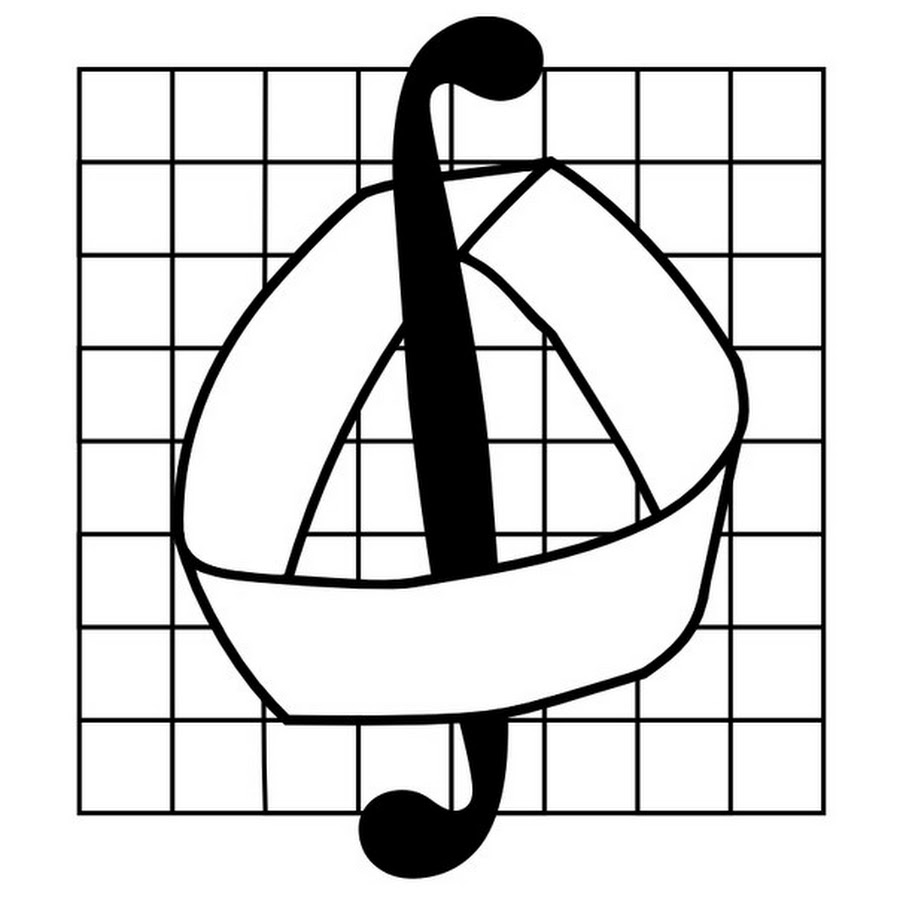
\includegraphics[width=0.30\linewidth]{emblema}
        \label{fig:emblema}
    \end{figure}
    \hfill \break
    \hfill \break
    \Large{\textbf{Курсовая работа}\\
        \hfill \break Модель восстановления человеком исходной позы после толчка
    }
\end{center}

\hfill \break
\hfill \break
\hfill \break
\begin{flushright}
    \large{
        Выполнил: студент группы М -- 1 \\ Романов Андрей Владимирович}
\end{flushright}

\begin{flushright}
    \large{
        Научный руководитель: к.ф.-м.н., \\ Кручинин Павел Анатольевич}
\end{flushright}
\hfill \break
\hfill \break
\begin{center} \large{Москва, 2022} \end{center}



\thispagestyle{empty} % выключаем отображение номера для этой страницы
\normalsize{
% КОНЕЦ ТИТУЛЬНОГО ЛИСТА
\newpage
\tableofcontents
\newpage

\section{Введение}
В ходе теста производят толкающее воздействие с помощью руки или
груза, помещенного на подвижном отвесе. В результате внешнего
воздействия тело наклоняется вперед и при не очень сильном толчке
человек не теряет равновесие и не падает, а возвращается в исходное
положение за счет изменения угла в голеностопном суставе. Изменение
остальных суставных углов может оказаться тоже не столь значительным.

В курсовой работе предполагается рассмотреть возможные оптимальные
алгоритмы управления изменением позы человека, основанные на модели
«перевернутого маятника», которые можно было бы использовать для
возвращения человека в исходную вертикальную позу. В дальнейшем
такое решение предполагается использовать для оценки времени
возвращения конкретного человека в вертикальную позу, сравнивая
его с полученным эталонным значением.
\newpage
\section{Математическая модель и постановка задачи управления}
Для описания движения тела человека в сагиттальной плоскости ис-пользуем традиционную модель перевернутого маятника (см. рисунок 1).

\begin{figure}[h!]
    \centering
    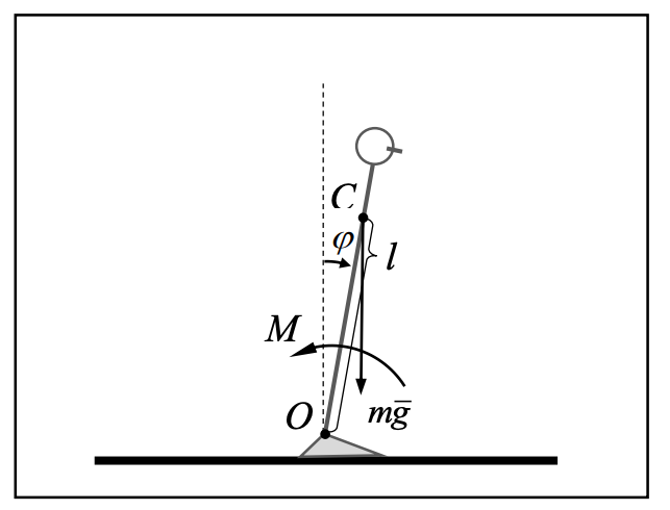
\includegraphics[width=1.00\linewidth]{pendulum.png}
    \caption{Модель перевернутого маятника}
    \label{fig:pendulum}
\end{figure}

Традиционно предполагаем, что тело человека в ходе теста допустимо
моделировать недеформируемым однородным стержнем массы $m$,
закрепленным шарнирно в точке $O$, которая соответствует
голеностопному суставу.

Центр масс стержня расположен в точке $C$, удаленной от точки $O$
на расстояние $l$. Момент инерции стержня относительно фронтальной
оси, проходящей через точку $O$, равен $J$. Отклонение стержня от
вертикали описывается углом $\varphi$. Будем считать, что обследуемый
ориентирован так, что его сагиттальная плоскость параллельна оси
чувствительности платформы, а его стопа неподвижна относительно
платформы. Момент $M$, который приложен в точке $O$ к стержню,
будем считать управлением.

Запишем уравнение моментов для малых значений угла $\varphi$ и
скорости его изменения запишем, как традиционно принято для этой задачи.
\begin{equation}\label{6}
    J\ddot{\varphi}= mgl\varphi+M
\end{equation}

Необходимо перевести решение уравнения из начального положения:
\begin{equation}\label{7}
    \varphi(0)=\varphi_0,\dot{\varphi}(0)=\omega_0.
\end{equation}

В конечное положение:
\begin{equation}\label{8}
    \varphi(t_k)=\varphi_k,\dot{\varphi}(t_k)=0.
\end{equation}

Перевод положения тела должен происходить за минимальное
время $t_k$, с помощью изменений значения момента $M$ в
голеностопном суставе.

Будем принимать во внимание условия ограниченности величины
момента в голеностопном суставе
\[
    M^-\le\ M\le\ M^+
\]
и скорости его изменения
\[
    U^-\le\dot{M}\le\ U^+.
\]

Будем считать, что за время толчка нервная система человека
не успела среагировать и момент в голеностопном суставе остался
неизменным, тогда:
\[
    M(0)=M\left(t_k\right)=-mgl\varphi_k;
\]

Для дальнейшего анализа задачи представим приведенные
соотношения в безразмерном виде. Для этого перейдем
к новым переменным:
\[
    \theta=\frac{\varphi-\varphi_f}{\varphi_\ast},\ \ m=\frac{M-M_f}{mgl\varphi}.
\]

В качестве характерного значения угла выберем разность
начального и конечного значений угла в голеностопном
суставе при выполнении пробы $\varphi_\ast=\varphi_0-\varphi_k$

Введем безразмерное время:
\[
    \tau=\frac{t}{t_\ast},\ t_\ast=\sqrt{\frac{J}{mgl}}.
\]

Управлением $u$ будем считать скорость изменения безразмерного
момента. Для этих переменных обезразмеренные уравнения движения
примут следующий вид:
\[
    \theta^{''}=\theta+m;\ m^{'}=u
\]

Здесь через $m^{'}$ обозначено дифференцирование по
безразмерному времени $\tau$. Необходимо решение системы
перевести из начального положения
\begin{equation}\label{9}
    \theta\left(0\right)=1;\ \dot{\theta}\left(0\right)=\frac{t_\ast}{\varphi_\ast}\omega_0;\ m\left(0\right)=0
\end{equation}
в положение
\begin{equation}\label{9}
    \theta\left(\tau_f\right)=0;\ \dot{\theta}\left(\tau_f\right)=0;\ m\left(\tau_f\right)=0
\end{equation}
с помощью ограниченного управления
\[
    u^-\le\ u\le\ u^+,\ where
\]
\[
    u^-=\frac{U^-}{mgl\varphi_\ast t_\ast},\ \ u^+=\frac{U^+}{mgl\varphi_\ast t_\ast}.
\]
\newpage
\section{Задача оптимального быстродействия при ограничении на величину скорости изменения момента}
Выпишем систему в форме Коши
\begin{equation}\label{koshisystem}
    \left\{ {\begin{aligned}
                 & \theta^{'} = \omega , \hfill   \\
                 & \omega^{'} = \theta+m , \hfill \\
                 & m^{'} = u . \hfill             \\
            \end{aligned}} \right.
\end{equation}
Проверим управляемость системы
\begin{equation*}
    A =
    \begin{pmatrix}
        0 & 1 & 0 \\
        1 & 0 & 1 \\
        0 & 0 & 0
    \end{pmatrix}
    b =
    \begin{pmatrix}
        0 \\
        0 \\
        1
    \end{pmatrix}
    W =
    \begin{pmatrix}
        0 & 0 & 1 \\
        0 & 1 & 0 \\
        1 & 0 & 0
    \end{pmatrix}
\end{equation*}
det $W\neq0$, значит система полностью управляемая

$|u|<U_{max}$
\[
    \theta(0)=1;\ \omega(0)=\frac{t_\ast}{\varphi_\ast}\omega_0;\ m(0)=0
\]
$\tau_f\to min$

Запишем функцию Понтрягина
\[
    H(\Psi(t),y(t),u(t))=\psi_1*\omega+\psi_2*(\theta+m)+\psi_3*u
\]
Сопряженная система уравнений:
\[
    \dot{\psi}_i  =  - \frac{{\partial H}}{{\partial y_i }},\,\,i = 1, \ldots ,n
\]
В данной задаче $y_1 = \theta, y_2 = \omega, y_3=m$, тогда сопряженная система примет вид
\begin{equation} \label{7}
    \left\{ {\begin{aligned}
                 & \dot \psi _\theta  =  - \frac{{\partial H}}{{\partial \theta}} = - \psi_2\hfill   \\
                 & \dot \psi _\omega   =  - \frac{{\partial H}}{{\partial \omega }} = - \psi_1\hfill \\
                 & \dot \psi _m   =  - \frac{{\partial H}}{{\partial m }} = - \psi_2 . \hfill        \\
            \end{aligned}} \right.
\end{equation}
При $\psi_3\equiv0$ следует, что $\psi_2\equiv0$ и $\psi_1\equiv0$, следовательно особого управления нет

Тогда для условия максимизации функции Понтрягина
\[
    u= 
\begin{cases}
    -U_{max},& \text{при $\psi_3<0$}\\
    -U_{min},& \text{при $\psi_3\geq0$}
\end{cases}
\]


\end{document}